\subsection{Number Systems}
  \begin{itemize}
    \setlength{\itemsep}{0em}
    \item \marginnote{4.5.1.1}The set of \textbf{natural numbers} are all positive whole numbers including 0.
      \subitem $ \mathbb{N}=\{0,1,2,3,...\} $
    \item \marginnote{4.5.1.2}The set of \textbf{integers} are all positive and negative whole numbers, including 0.
      \subitem $ \mathbb{Z}=\{...,-3,-2,-1,0,1,2,3,...\} $
    \item \marginnote{4.5.1.3}The set of \textbf{rational numbers} is the set of all numbers that can be expressed as the ratio of two integers.
      \subitem $ \mathbb{Q} $
    \item \marginnote{4.5.1.4}The set of \textbf{irrational numbers} is the set of all numbers that cannot be expressed as the ratio of two integers.
    \item \marginnote{4.5.1.5}The set of \textbf{Real numbers} is the set made by combining the rationals with the irrationals. It's the set of all "possible real world possibilities"
      \subitem $ \mathbb{R} $
    \item \marginnote{4.5.1.6}\textbf{Ordinals} are numbers used to identify the position relative to other numbers. For example, use of \textit{First}, \textit{Second}, \textit{Third}, etc, is essentially use of ordinal numbers.
  \end{itemize}
  \marginnote{4.5.1.7}We are use to using natural and real numbers in every day life, as we use natural numbers to count objects, and real numbers for measurements.
\subsection{Number bases}
  \noindent
  \marginnote{4.5.2.1}A number base indicates the number of digits available within a system, e.g. base 10 for decimal, base 2 for binary. The accepted method for representing different number bases is by using subscript numbers to represent their base. e.g:
  \begin{itemize}
    \setlength{\itemsep}{0em}
    \item $ 67_{10} $ Decimal (base 10)
    \item $ 10011011_2 $ Binary (base 2)
    \item $ \textrm{AE}_{16} $ Hexadecimal (base 16)
    \subitem Hexadecimal is useful because it allows us to represent large numbers with less digits, e.g: $ 1101001_2 = 211_{10} = \textrm{D}3_{16} $. Through some calculations, you can show that binary number of length $ n $ will be converted to a decimal number of length $ \log_{10}{(2)}n $ which will be converted to a hexadecimal number of length $ \frac{n}{4} $. This means that 8 bits (= 1 byte) can be written as two hex digits. This is also the reason why hexadecimal is used to show memory addresses and colour codes.
  \end{itemize}
  \begin{table}[H]
    \centering
    \begin{tabular}{ C{3cm} C{3cm} C{3cm} }
      Decimal & Binary & Hexadecimal\\
      1 & 1 & 1 \\
      2 & 10 & 2 \\
      3 & 11 & 3 \\
      4 & 100 & 4 \\
      5 & 101 & 5 \\
      6 & 110 & 6 \\
      7 & 111 & 7 \\
      8 & 1000 & 8 \\
      9 & 1001 & 9 \\
      10 & 1010 & A \\
      11 & 1011 & B \\
      12 & 1100 & C \\
      13 & 1101 & D \\
      14 & 1110 & E \\
      15 & 1111 & F \\
      16 & 10000 & 10 \\
    \end{tabular}
  \end{table}
  Here are a list of conversions which you need to be comfortable with:
  \begin{itemize}
    \setlength{\itemsep}{0em}
    \item Binary $ \to $ Decimal
      \begin{enumerate}
        \setlength{\itemsep}{0em}
        \item Write down the binary number with spaces between each bit.
        \item Above the Least significant bit write the number 1.
        \item As you move left from the LSB, double the value of the previous number.
        \item Wherever there's a one on the bottom, add those decimal values together.
      \end{enumerate}
      \subitem For Example:
      \begin{table}[h]
        \centering
        \begin{tabular}{ C{1cm} C{1cm} C{1cm} C{1cm} C{1cm} C{1cm} C{1cm} C{1cm} }
        $ 2^7 = 128 $ & $ 2^6 = 64 $ & $ 2^5 = 32 $ & $ 2^4 = 16 $ & $ 2^3 = 8 $ & $ 2^2 = 4 $ & $ 2^1 = 2 $ & $ 2^0 = 1 $ \\
        \hline
        $ 1 $ & $ 1 $ & $ 0 $ & $ 0 $ & $ 1 $ & $ 1 $ & $ 1 $ & $ 1 $ \\
        \end{tabular}
      \end{table}
      \subitem $ 11001111_2 = 128 + 64 + 8 + 4 + 2 + 1 = 207 $
    \item Decimal $ \to $ Binary
      \begin{enumerate}
        \item Divide by two and note down the remainder until you get the result 0 remainder 0.
        \item reverse the order in which you noted down the remainders. For example:
        \begin{align*}
          & 207/2 & = & 103 & & \textrm{remainder} & \textbf{1}\\
          & 103/2 & = & 51 & & \textrm{remainder} & \textbf{1}\\
          & 51/2 & = & 25 & & \textrm{remainder} & \textbf{1}\\
          & 25/2 & = & 12 & & \textrm{remainder} & \textbf{1}\\
          & 12/2 & = & 6 & & \textrm{remainder} & \textbf{0} \\
          & 6/2 & = & 3 & & \textrm{remainder} & \textbf{0} \\
          & 3/2 & = & 1 & & \textrm{remainder} & \textbf{1} \\
          & 1/2 & = & 0 & & \textrm{remainder} & \textbf{1} \\
          & 0/2 & = & 0 & & \textrm{remainder} & \textbf{0}
        \end{align*}
      \end{enumerate}
      \subitem $ 207_{10} = 11001111_{16} $
    \item Hexadecimal $ \to $ Decimal
      \begin{enumerate}
        \setlength{\itemsep}{0em}
        \item Write down the hexadecimal number with spaces between each hex digit.
        \item Beneath each hex digit, write down the decimal equivalent.
        \item Above the Least significant bit write the number 1.
        \item As you move left from the LSB, multiply the value by 16 the value of the previous number.
        \item multiply the value in the bottom row with the corresponding value in the top row, add these decimal values together.
      \end{enumerate}
      \subitem For Example:
      \begin{table}[h]
        \centering
        \begin{tabular}{ C{1cm} C{1cm} C{1cm} }
          $ 16^2 = 256 $ & $ 16^1 = 16 $ & $ 16^0 = 1 $ \\
          \hline
          $ 9 $ & $ 0 $ & $ A $ \\
          $ 9 $ & $ 0 $ & $ 10 $
        \end{tabular}
      \end{table}
      \subitem $ 90\textrm{A}_{16} = 9 \times 256 + 0 \times 16 + 10 \times 1 = 2314_{10} $
    \item Decimal $ \to $ Hexadecimal
      \begin{enumerate}
        \item Divide by 16 and note down the remainder until you get the result 0 remainder 0.
        \item Convert the remainders to hex digits.
        \item reverse the order in which you noted down the remainders. For example:
        \begin{align*}
          & \textbf{2314}/16 & = & 144 & & \textrm{remainder} & 10 & & \textbf{A}\\
          & 144/16 & = & 9 & & \textrm{remainder} & 0 & & \textbf{0}\\
          & 9/16 & = & 0 & & \textrm{remainder} & 9 & & \textbf{9}\\
          & 0/16 & = & 0 & & \textrm{remainder} & 0 & & \textbf{0}
        \end{align*}
      \end{enumerate}
      \subitem $ 2314_{10} = 90\text{A}_{16} $
    \item Binary $ \to $ Hexadecimal
      \begin{enumerate}
        \item Write out the binary number, splitting it into blocks of four from the right.
        \item Convert each of the binary blocks into hexadecimal (which can be done via a conversion to decimal)
        \item Stick all of the blocks together to make one hexadecimal number.
        \begin{table}[H]
          \centering
          \begin{tabular}{ c c c c }
            1100 & 1010 & 1110 & 0111 \\
            12 & 10 & 14 & 7 \\
            C & A & E & 7
          \end{tabular}
        \end{table}
      \end{enumerate}
      \subitem $ 1100101011100111_2 = \text{CAE}7_{16} $
    \item Hexadecimal $ \to $ Binary
      \begin{enumerate}
        \setlength{\itemsep}{0em}
        \item Write out the hexadecimal number with spaces between each digit.
        \item Convert each digit from hexadecimal to binary, which can be done via decimal, or just remembering how each binary number convert to hex digits. MAKE SURE ALL THE BLOCKS ARE FOUR DIGITS LONG.
        \item Put all the blocks of binary numbers together to form the binary number
        \begin{table}[H]
          \centering
          \begin{tabular}{ c c c c }
            C & A & E & 7 \\
            12 & 10 & 14 & 7 \\
            1100 & 1010 & 1110 & 0111
          \end{tabular}
        \end{table}
      \end{enumerate}
      \subitem $ \text{CAE}7_{16} = 1100101011100111_2 $
  \end{itemize}
\subsection{Units of Information}
  \marginnote{4.5.3.1}A binary digit (bit) is the fundamental unit of information, and can take the value 0 or 1. due to the fact that one byte can only store 2 possible values (0 or 1), bytes are more often used which consist of 8 bits (meaning they can store 256 different values). We can calculate the number of different values which can be obtained from using $n$ bits by calculating $2^n$. From this we can see that
  \begin{itemize}
    \setlength{\itemsep}{0em}
    \item If we use 3 bits, we can get $2^3=8$ different values.
    \item if we use 8 bits (1 byte), we can get $2^8=256$ different values.
    \item if we use 16 bits (2 bytes), we can get $2^{16}=65,536$ different values.
    \item if we use 32 bits (4 bytes), we can get $2^{32}=4,294,967,296$ different values.
  \end{itemize}
  \marginnote{4.5.3.2}A unit describes a grouping of bits, for example one byte is unit of 8 bits. You can use prefixes to dictate the size of a unit. The prefixes used fall into the categories of binary and decimal, because binary prefixes can be written as $2^n$ whereas decimal prefixes can be written as $10^n$, these prefixes are approximately equal because $2^{10} \approxeq 10^3 \implies 1024 \approxeq 1000 $. All the prefixes we need to know are:
  \begin{table}[H]
    \begin{tabular}{ l l c | l l c }
      \multicolumn{3}{ l |}{Binary} & \multicolumn{3}{ l }{Decimal} \\
      \hline
      Kibi & Ki & $2^{10}$ & Kilo & K & $10^3$ \\
      Mebi & Ki & $2^{20}$ & Mega & K & $10^6$ \\
      Gibi & Ki & $2^{30}$ & Giga & K & $10^9$ \\
      Tebi & Ki & $2^{40}$ & Tera & K & $10^{12}$ \\
    \end{tabular}
  \end{table}
\subsection{Binary Number System}
  \noindent
  \marginnote{4.5.4.1}Unsigned binary numbers are binary numbers that have no sign, they are all positive. On the other hand, signed binary numbers are numbers that do have a sign, they can be positive or negative. We know from above that is an unsigned binary number has n bits, it can represent $2^n$ values, meaning it could represent the values $1 \to 2^n$ however, if we want the first binary number it represents to be 0, then the range of values n bits can represent is $0 \to 2^n-1$.\\
  \marginnote{4.5.4.2}To form binary addition we can simply perform column addition. For example, to do $11000101_2 + 10100011_2$ we would do:
  \begin{table}[H]
    \begin{tabular}{ c@{\,} c@{\,} c@{\,} c@{\,} c@{\,} c@{\,} c@{\,} c@{\,} c@{\,} }
      & 1 & 1 & 0 & 0 & 0 & 1 & 0 & 1 \\
      $+$& 1 & 0 & 1 & 0 & 0 & 0 & 1 & 1 \\ \hline
      1 & 0 & 1 & 1 & 0 & 1 & 0 & 0 & 0 \\ \hline
      $^1$&   &   &   &   &$^1$&$^1$&$^1$&
    \end{tabular}
  \end{table}
  We can do the something similar for multiplication, in that we perform column multiplication. For example, to do $100101_2 \times 101_2$ we would do:
  \begin{table}[H]
    \begin{tabular}{ c@{\,} c@{\,} c@{\,} c@{\,} c@{\,} c@{\,} c@{\,} c@{\,} c@{\,} }
        &     &     &  1  &  0  &  0  &  1  &  0  &  1  \\
      $\times$&     &     &     &     &     &  1  &  0  &  1  \\ \hline
        &     &     &  1  &  0  &  0  &  1  &  0  &  1  \\
      $  +   $&  1  &  0  &  0  &  1  &  0  &  1  &  0  &  0  \\ \hline
        &  1  &  0  &  1  &  1  &  1  &  0  &  0  &  1  \\ \hline
        &     &     &     &     &$^1$ &     &     &     \\
    \end{tabular}
  \end{table}
  \noindent
  \marginnote{4.5.4.3}As said above signed binary numbers can be used to represent both positive and negative numbers, one possible way of coding this is by using two's complement. Within two's complement if you decide to use n bits, then the range of values that can be used is $-2^{n-1} \to 2^{n-1}-1$. To convert a binary two's complement to decimal, we do a similar method to convert an unsigned binary number to decimal, except we make the most significant bit negative, for example:
  \begin{table}[H]
    \centering
    \begin{tabular}{ C{1cm} C{1cm} C{1cm} C{1cm} C{1cm} C{1cm} C{1cm} C{1cm} }
      $ 2^7 = -128 $ & $ 2^6 = 64 $ & $ 2^5 = 32 $ & $ 2^4 = 16 $ & $ 2^3 = 8 $ & $ 2^2 = 4 $ & $ 2^1 = 2 $ & $ 2^0 = 1 $ \\
      \hline
      $ 1 $ & $ 1 $ & $ 0 $ & $ 0 $ & $ 1 $ & $ 1 $ & $ 1 $ & $ 1 $ \\
    \end{tabular}
  \end{table}
  \noindent
  $11001111_2 = -128+64+8+4+2+1 = -49_{10}$ \\
  To convert a positive integer into a two's complement, you simply use the method to convert a decimal number to binary, making sure the MSB is zero. To convert a negative integer into a two's complement, you do the following:
  \begin{itemize}
    \setlength{\itemsep}{0em}
    \item Make the number positive (e.g. $-58\to58$ )
    \item Convert the positive number into a positive two's complement (as described above)
    \item Starting from the LSB, working to the left, write down all the digits including the first 1 you come across.
    \item After the first 1, reverse all of the bits ($1\to0$, $0\to1$)
  \end{itemize}
  For example:\\
  $-49_{10}\to49_{10}$\\
  $49_{10} = 0110001_2$\\
  $-49_{10}=1001111_2$\\
  To perform subtraction you simply convert one of the numbers into two's complement. For example: \\
  $ 102_{10} - 73_{10} = 01100110_2 - (01001001_2) $\\
  $-01001001_2=10110111_2 \implies 01100110_2 - 01001001_2 = 01100110_2 + 10110111_2 $
  \begin{table}[H]
    \begin{tabular}{ c@{\,} c@{\,} c@{\,} c@{\,} c@{\,} c@{\,} c@{\,} c@{\,} c@{\,} }
     &  0  &  1  &  1  &  0  &  0  &  1  &  1  &  0  \\
      $ + $&  1  &  0  &  1  &  1  &  0  &  1  &  1  &  1  \\ \hline
    1  &  0  &  0  &  0  &  1  &  1  &  1  &  0  &  1  \\ \hline
      $^1$ & $^1$& $^1$&     &     & $^1$& $^1$&     &
    \end{tabular}
  \end{table}
  \noindent
  $ 01100110_2 - (01001001_2) = 00011101_2 = 29_{10} $\\
  \marginnote{4.5.4.4}Numbers with a fractional part can be represented in many ways, one way to represent them is using fixed point binary numbers. This method means that the binary is in a fixed place and the programmer can determine how many are before and after the binary point. Conversion from binary (signed or unsigned) to decimal is similar to always, except you place the one before the decimal place, doubling as you go to the left, and halving as you move right. To convert from decimal to binary, you can break it into two parts:
  \begin{enumerate}
    \setlength{\itemsep}{0em}
    \item The part before the binary point (the integer)
    \item The part after the binary point (the fraction)
  \end{enumerate}
  You can deal with part 1 by simply using the original method to convert from decimal to binary, to deal with part 2, you will have to try and seperate the fraction to show it as the sum of fractions in the form $ \frac{1}{2^n} $.
  
  \noindent
  \marginnote{4.5.4.5}Rounding Errors
  
  \noindent
  \marginnote{4.5.4.6}Absolute and Relative Errors
  
  \noindent
  \marginnote{4.5.4.7}Range and Precision
  
  \noindent
  \marginnote{4.5.4.8}Normalisation of Floating Point Form
  
  \noindent
  \marginnote{4.5.4.9}Underflow and Overflow
  
\subsection{Information Coding Systems}
  \noindent
  \marginnote{4.5.5.1}When using character codes (which are binary codes that represent different characters) We need to realise that the binary representation of $9_{10}$ does not equal $1001_2$ but has a completely different value, due to the fact it is representing the character "9", not the value of 9. \\
  \marginnote{4.5.5.2}Before standardised coding systems, different programs would use different character codes for each character, which made it harder to understand different programs as they may use completely different character codes to represent the same character.\\
  For this reason, ASCII (American Standard Code for Information Interchange) was invented to create a standard for all the keys on a keyboard. ASCII uses 7 bits meaning it could show 128 different characters, extended ASCII uses 8 bits meaning it could show 256 different characters.\\
  ASCII has many limitation:
  \begin{itemize}
    \setlength{\itemsep}{0em}
    \item It only allows a maximum of 256 characters, which isn't sufficient to store all possible and necessary characters, numbers and symbols.
    \item It was initially developed in English, so it doesn't represent other languages and scripts of the world.
    \item Worldwide use of the internet made a universal international coding system more important.
    \item The range of platforms and programs has drastically increased, meaning developers from around the world are using a wider range of characters.
  \end{itemize}
  Because of this, a new standard was created called Unicode. Unicode is a superset of ASCII (or you could say ASCII was subsumed by Unicode) meaning for the first 256 characters (8 bits), the two are the same. For example in ASCII the character code for "A" is 65 so in Unicode the character code for "A" is also 65. Unicode comes in two different forms UTF-8 which uses 8 bits, and therefore resembles extended ASCII, and UTF-16 which uses 16 bits, meaning it can store 65536 different characters, making it very useful for storing all characters worldwide.\\
  \marginnote{4.5.5.3}There are several ways of checking whether a sequence of bits has an error. Three ways of doing this are:
  \begin{itemize}
    \setlength{\itemsep}{0em}
    \item Parity Bit
      \subitem This is a method of checking binary codes by counting the number of 0s and 1s in the code, parity always depends on the number of 1s in a number. There are 2 different types of parities
      \begin{itemize}
        \setlength{\itemsep}{0em}
        \item Even Parity
          \subitem This process makes sure there are an even number of 1s in the number. This means that if there are an odd number of 1s within the number, the parity bit will be 1, but if there are an even number of 1s, then the parity bit will be 0.
        \item Odd Parity
          \subitem This process makes sure there are an odd number of 1s in the number. This means that if there are an odd number of 1s within the number, the parity bit will be 0, but if there are an even number of 1s, then the parity bit will be 1.
      \end{itemize}
    \item Majority Voting
      \subitem This is a method of checking binary codes via producinng the same data serveral (3) times and taking the majority. So for example if you wanted to send the data 1001, we would send the data 111000000111, however due to possible interferences the actual data sent may be 101001000111. We can split the data into blocks of three and we get
      \begin{itemize}
        \setlength{\itemsep}{0em}
        \item 101 $\to$ 1
        \item 001 $\to$ 0
        \item 000 $\to$ 0
        \item 111 $\to$ 1
      \end{itemize}
      \subitem meaning we get the final datum of 1001.
    \item Check Digits
      \subitem This has many uses outside of binary, the central idea is that a digit is added to the end of the number, which is the result of some sort of simple arithmetic calculation, this calculation can then be done again at the other end to check whether the number transmitted is valid. A system using weights is often used as it usually means that both changing values and translation (the position of numbers changing)
  \end{itemize}
\subsection{Representing Images, Sound and Other Data}
  \noindent
  \marginnote{4.5.6.1}Different patterns of bits can be used to represent different forms of data for example, in an image each pixel may be given 3 bytes (1 byte for red, 1 byte for green, 1 byte for blue), whereas a sound may use 1 byte to represent an amplitude every set time period (e.g. every 0.01 seconds).\\
  \marginnote{4.5.6.2}Analogue data are data that are infinitely variable and are often represented in the form of a wave, for example a sound wave, whereas digital data are often represented by discrete values (often 1 and 0). Analogue signals are signals that can vary in both frequency and amplitude whereas digital signals is described as using binary (0s and 1s), and therefore, cannot take on any fractional values.\\
  \marginnote{4.5.6.3}There are two main conversion to do with audio:
  \begin{itemize}
    \setlength{\itemsep}{0em}
    \item Analogue to Digital Converter
      \subitem An ADC works by taking a series of readings are taken from the wave at fixed intervals in order to create discrete data values, which can be easily converted to binary. These readings can then be stored as binary codes. This is called sampling because you don't take the reading every time the amplitude changes, instead you use set points.
    \item Digital to Analogue Converter
      \subitem A DAC is usually embedded in a device that plays the audio data and signal is passed in analogue form to the loudspeaker or headphones, which then play the audio out loud.
  \end{itemize}
  \marginnote{4.5.6.4}Bit-mapped graphics are images made up of individual pixels, with each pixel being represented by a set number of bits. A pixel is an individual picture element. Resolution is width (of image in pixels) $\times$ height (of image in pixels). Colour depth is the number of bits allocated to represent the colour of a pixel in a bit-mapped graphic. We can also calculate the number of pixels per inch (PPI) by dividing the number of pixels in a given direction, by the length of the screen in that direction. For example a monitor that is 12 $\times$ 9 image with resolution 1366 $\times$ 768. The PPI in the horizontal axis would be $\frac{1366}{12}\approxeq114$ PPI and the PPI in the vertical axis would be $\frac{768}{9}\approxeq85$ PPI.\\
  We can calculate the amount of storage a picture needs by first finding out the number of pixels a picture is made up of (the resolution) and then multiplying this by the number of bits used to represent each pixel (colour depth), so we end up with the formulas: Storage = resolution $\times$ Colour Depth \\
  We also need to note that the picture may also contain meta data, meaning that the bit-map stores information about itself, such as width, height, colour depth, file type, and this will add to the size of the file. The meta data will normally be found at the beginning of a file within the header.\\
  
  \noindent
  \marginnote{4.5.6.5}Vector Graphics
  
  \noindent
  \marginnote{4.5.6.6}Vector Graphics versus Bitmapped Graphics
  
  \marginnote{4.5.6.7}The sample rate of a sound represents the number of samples that will be taken per second, the higher the sample rate, the more accurate the sound will be compared to the original analogue sound. The sampling resolution is the number of bits allocated to representing the (amplitude of the) sound. When deciding the optimum sampling rate, many programmers refer to Nyquist's Theorem, which states that to faithfully recreate the analogue signal, you should sample at least twice the highest frequency for example, the human ear can hear a maximum frequency of 20,000Hz, so a sampling rate of at least 40,000Hz should be used. This is because using double the frequency allows the sample to cover the complete range of peaks and troughs. To calculate the space a sound sample will take up, we do the following calculation: Sample rate (Hz) $\times$ length of recording (seconds) $\times$ sampling resolution (bits)\\
  \marginnote{4.5.6.8}Musical Instrument Digital Interface (MIDI) is a way to convert Analogue signals from instruments to digital signals. MIDI uses event messages to control various properties of the sound. These messages provide communication between MIDI devices or between a MIDI device and a processor. For Example, an event message may contain data on:
  \begin{itemize}
    \setlength{\itemsep}{0em}
    \item When to play a note
    \item When to stop playing a note
    \item Timing a note to play with other notes or sounds
    \item Timing a note to play with other MIDI-enabled devices
    \item What pitch a note is
    \item How loud to play it
    \item What effect to use when playing it
  \end{itemize}
  The advantage of using midi files over other digital audio formats are:
  \begin{itemize}
    \setlength{\itemsep}{0em}
    \item MIDI files tend to be smaller
    \item MIDI files are completely editable as individual elements and sounds can be selected and edited
    \item MIDI supports a wide range of instruments, providing more choices for music production
    \item MIDI files can produce very high quality authentic reproduction of the instrument
  \end{itemize}
  \marginnote{4.5.6.9}Often we find that files can be extremely large, taking up megabytes or gigabytes of space. Compression is the process of reducing the number of bits required to represent data, this is useful for making files smaller, which in turn makes the files easier to transmit.\\
  Lossless compression is compression where all the data is kept (no data is lost), the compressed is as accurate as the uncompressed file. Lossy compression is compression that causes some degradation in the quality of the file, for example, a grainier photo.\\
  Two of the methods used for lossless compression are as follows:
  \begin{itemize}
    \setlength{\itemsep}{0em}
    \item Run Length Encoding (RLE)
    \subitem This method compresses data by eliminating repeated data, for example, NNNNNN $\to$ 6N.
    \item Dictionary-Based Methods
    \subitem This method is used to compress data files by using a dictionary to associate certain groupings of characters with a certain token, as shown below, so to create the string "creation" we would simply use 41.
    \begin{table}[H]
      \centering
      \begin{tabular}{ l | c }
        Data & Token \\ \hline
        tion & 1 \\
        sta & 2 \\
        na & 3 \\
        crea & 4
      \end{tabular}
    \end{table}
  \end{itemize}
  \marginnote{4.5.6.10}Encryption is the process of turning plaintext (A normal piece of text) into scrambled ciphertext, which can only be understood if decrypted. A key in encryption is a piece of data used that defines the way in which plaintext is converted into ciphertext and therefore implies how to convert ciphertext to plaintext. There are many ciphers that can be used when to encrypt data, Two examples are:
  \begin{itemize}
    \setlength{\itemsep}{0em}
    \item Caesar Cipher
    \subitem The caesar cipher is a substitution cipher where one character of plaintext is substituted for another, which becomes the cipher text. This works by shifting all of the letters in the cipher text backwards or forwards a certain amount along the Alphabet, the amount shifted is dictated by the key. For example, if you were to use a key of 2 A$\to$C, B$\to$D, C$\to$E, ...etc.
    \begin{table}[H]
      \centering
      \begin{tabular}{|c@{\,}|c@{\,}|c@{\,}|c@{\,}|c@{\,}|c@{\,}|c@{\,}|c@{\,}|c@{\,}|c@{\,}|c@{\,}|c@{\,}|c@{\,}|c@{\,}|c@{\,}|c@{\,}|c@{\,}|c@{\,}|c@{\,}|c@{\,}|c@{\,}|c@{\,}|c@{\,}|c@{\,}|c@{\,}|c@{\,}|} \hline
        A & B & C & D & E & F & G & H & I & J & K & L & M & N & O & P & Q & R & S & T & U & V & W & X & Y & Z \\ \hline
        C & D & E & F & G & H & I & J & K & L & M & N & O & P & Q & R & S & T & U & V & W & X & Y & Z & A & B\\ \hline
      \end{tabular}
    \end{table}
    \subitem The caesar cipher is one of the easiest due to the fact that you can do simple frequency analysis of the cipher text as all you would see is a shift in the frequency of certain letters, and can therefore see what the key was for the cipher and undo the cipher.\\
    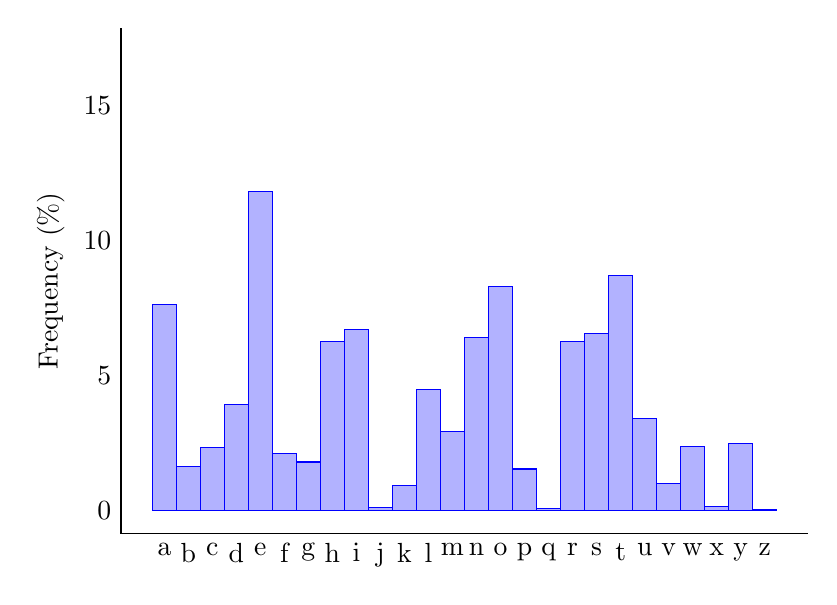
\begin{tikzpicture}
      \begin{axis}[
        xtick=data,
        tickwidth = 0pt,
        ylabel=Frequency (\%),
        width  = 0.85*\textwidth,
        height = 8cm,
        enlargelimits=0.05,
        ybar interval=1,
        ymax=17,
        xmajorgrids = false,
        axis lines*=left,
        symbolic x coords={a,b,c,d,e,f,g,h,i,j,k,l,m,n,o,p,q,r,s,t,u,v,w,x,y,z,aa},
        ]
        \addplot
        coordinates { (a, 7.6274260239915055) (b, 1.6343240765776164) (c, 2.3262132592968734) (d, 3.9426261400581657) (e, 11.796698694909553) (f, 2.123914348081273) (g, 1.799006838700317) (h, 6.248290324920699) (i, 6.6999479018972945) (j, 0.12606421915495558) (k, 0.9340200610668901) (l, 4.484894847563589) (m, 2.9399684773505146) (n, 6.416956283756603) (o, 8.298766132276423) (p, 1.5422093552365188) (q, 0.09448881209731134) (r, 6.274563595956133) (s, 6.568027592210345) (t, 8.699064212560259) (u, 3.4014653415723073) (v, 0.9910246180022027) (w, 2.357999696643959) (x, 0.13964929403773485) (y, 2.489366051821125) (z, 0.043023800259831046)  (aa,0) };
      \end{axis}
    \end{tikzpicture}
    \item Vernam Cipher/ One-time Pad
    \subitem The Vernham cipher is a method of encryption that uses a one-time pad (key) to create ciphertext. the one time pad is a randomly generated string with the same length as the cipher text. To encrypt a message, each character in the plaintext is combined with the character at the corresponding position in the key by converting them into a binary code and performing a bitwise xor on the binary representations to obtain new binary codes, which can in turn be mapped to new characters. So For example
    \begin{table}[H]
      \centering
      \begin{tabular}{c|c|c|c|c|c|} \cline{2-6}
        Plaintext Message & H & E & L & L & O \\ \cline{2-6}
        Key & I & S & W & I & B \\ \cline{2-6}
        Ciphertext & L & & E & H & E \\ \cline{2-6}
      \end{tabular}
    \end{table}
  \end{itemize}
  The Vernham is said to be mathematically impossible to crack, this is due to the fact that a random key is used, meaning that all characters have an equal chance of appearing, so no form of analysis can be done to figure out what the key is, and thus is impossible to get the original message. This is different to other cyphers which may be computationally secure, meaning that they can theoretically be solved with enough time and cipher text, but not in any time that would be considered useful using current technology.
